\section{\texorpdfstring{
\includegraphics[width=100pt]{webpack.png}}{Webpack}}

\begin{frame}
  \frametitle{Webpack}
  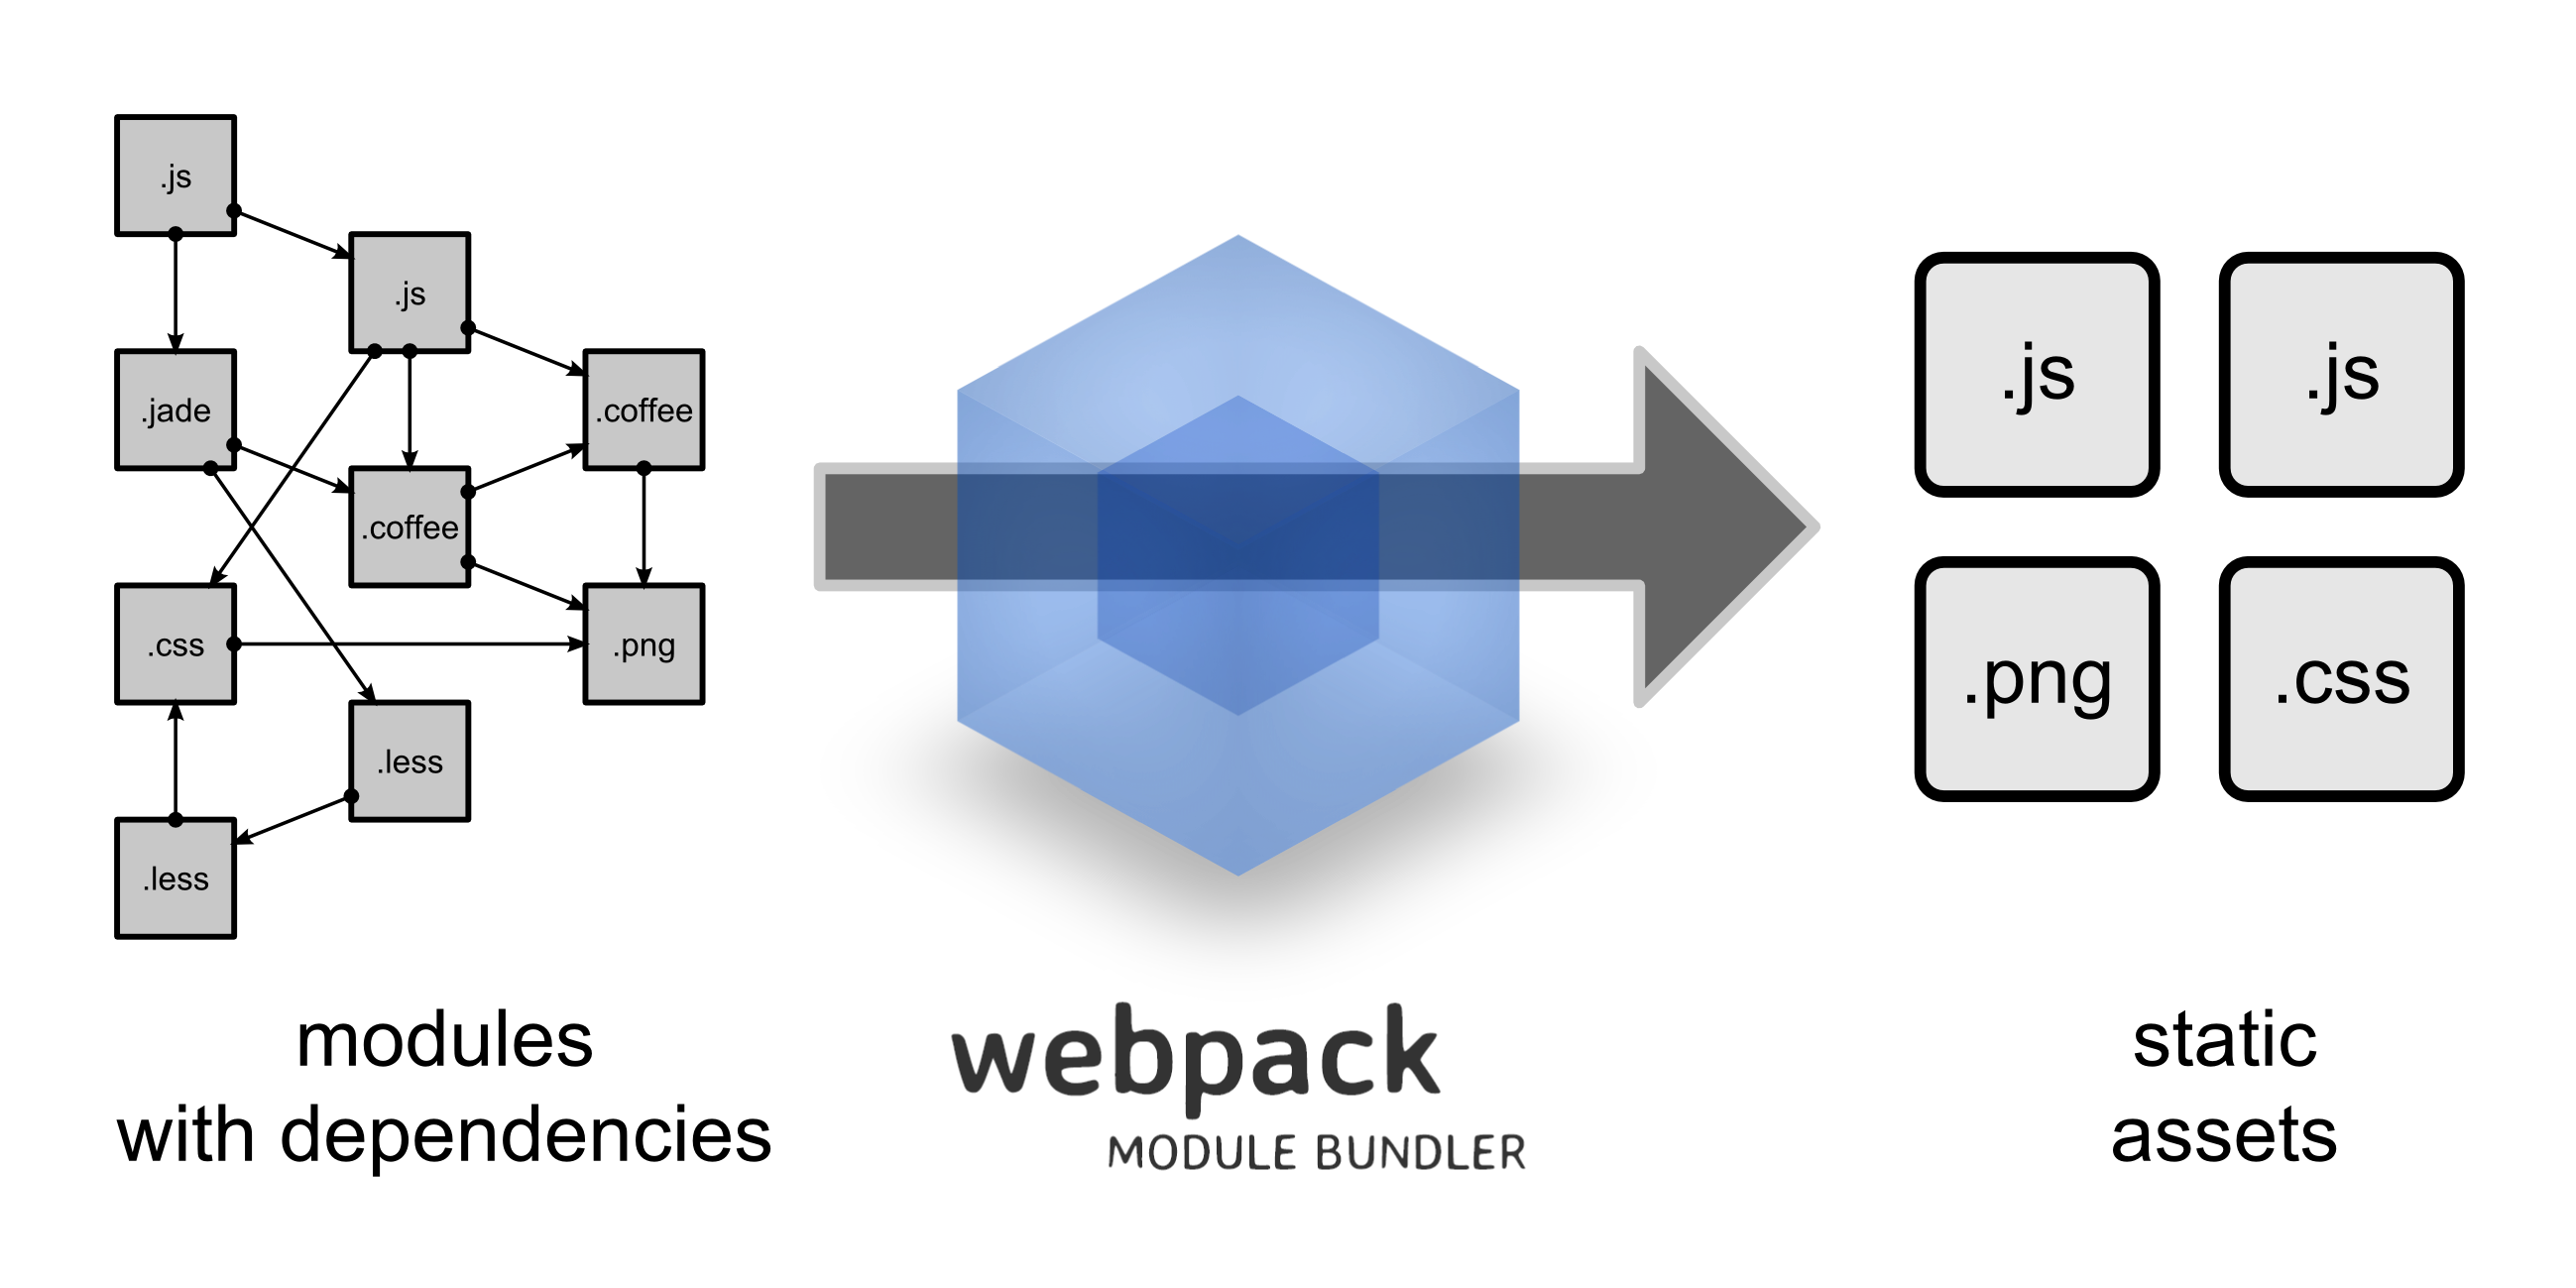
\includegraphics[width=\textwidth]{what-is-webpack.png}
\end{frame}

\begin{frame}
  \frametitle{Loaders}
  Webpack can only process JavaScript natively, but loaders are used to transform other resources into JavaScript. By doing so, every resource forms a module.

  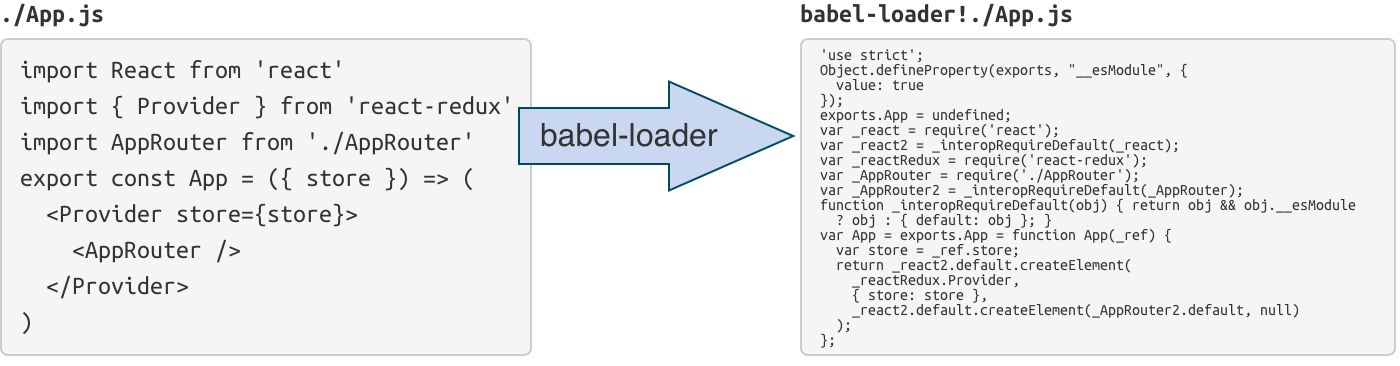
\includegraphics[width=\textwidth]{babel-loader}

  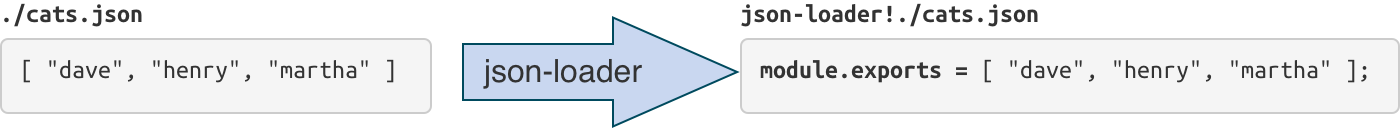
\includegraphics[width=\textwidth]{json-loader}
\end{frame}

\begin{frame}[fragile]
  \frametitle{Config}
  \begin{minted}[fontsize=\tiny]{javascript}
  module.export = {
    devtool: 'source-map',
    entry: {
      app: '/path/to/entry_file.js',
    },
    output: {
      path: '/path/to/destination/folder/',
      filename: '[name]-[hash].js'  // Creates a file app-e5fb0d5a9741647e0223.js
    },
    module: {
      loaders: [
        {
          test: /\.jsx?$/,  // For matching file names
          loaders: [ 'babel?cacheDirectory' ],
          include: [ 'scr/path/js/', 'scr/path/jsx' ]  // Path to search
        },
        {
          test: /\.scss$/,
          loaders: [ 'style', 'css', 'sass' ]
        }
      ]
    },
    plugins: [
      new webpack.DefinePlugin({
        'process.env': { 'NODE_ENV': JSON.stringify('production') }
      }),
    ]
  }
  \end{minted}
\end{frame}

\begin{frame}[fragile]
  \frametitle{Executing webpack}
  \begin{minted}[fontsize=\tiny]{javascript}
{
  "name": "crashui",
  "version": "1.0.0",
  "dependencies": {
    "babel-core": "^6.11.4",
    "react": "^15.2.1",
    "react-dom": "^15.2.1",
    "redux": "^3.5.2",
    ...
  },
  "devDependencies": {
    "babel-loader": "^6.2.4",
    "babel-preset-es2015": "^6.9.0",
    "babel-preset-stage-0": "^6.5.0",
    "clean-webpack-plugin": "^0.1.10",
    "standard": "^7.1.2",
    "standard-loader": "^4.0.0",
    "webpack": "^1.13.1",
    "webpack-dev-server": "^1.14.1",
    ...
  },
  "scripts": {  // Commands run in terminal. Ex: npm run build
    "build": "NODE_ENV=production webpack --config config/webpack.config.js",
    "lint": "standard \"frontend/**/*.js*\" --verbose | snazzy",
    "start": "NODE_ENV=development webpack-dev-server --config config/webpack.config.js",
    "test": "NODE_ENV=testing karma start"
  },
}
  \end{minted}
\end{frame}
